\documentclass[tikz,border=20pt]{standalone}
\usepackage{tikz}
\usetikzlibrary{shapes.geometric, arrows.meta, positioning}

\begin{document}
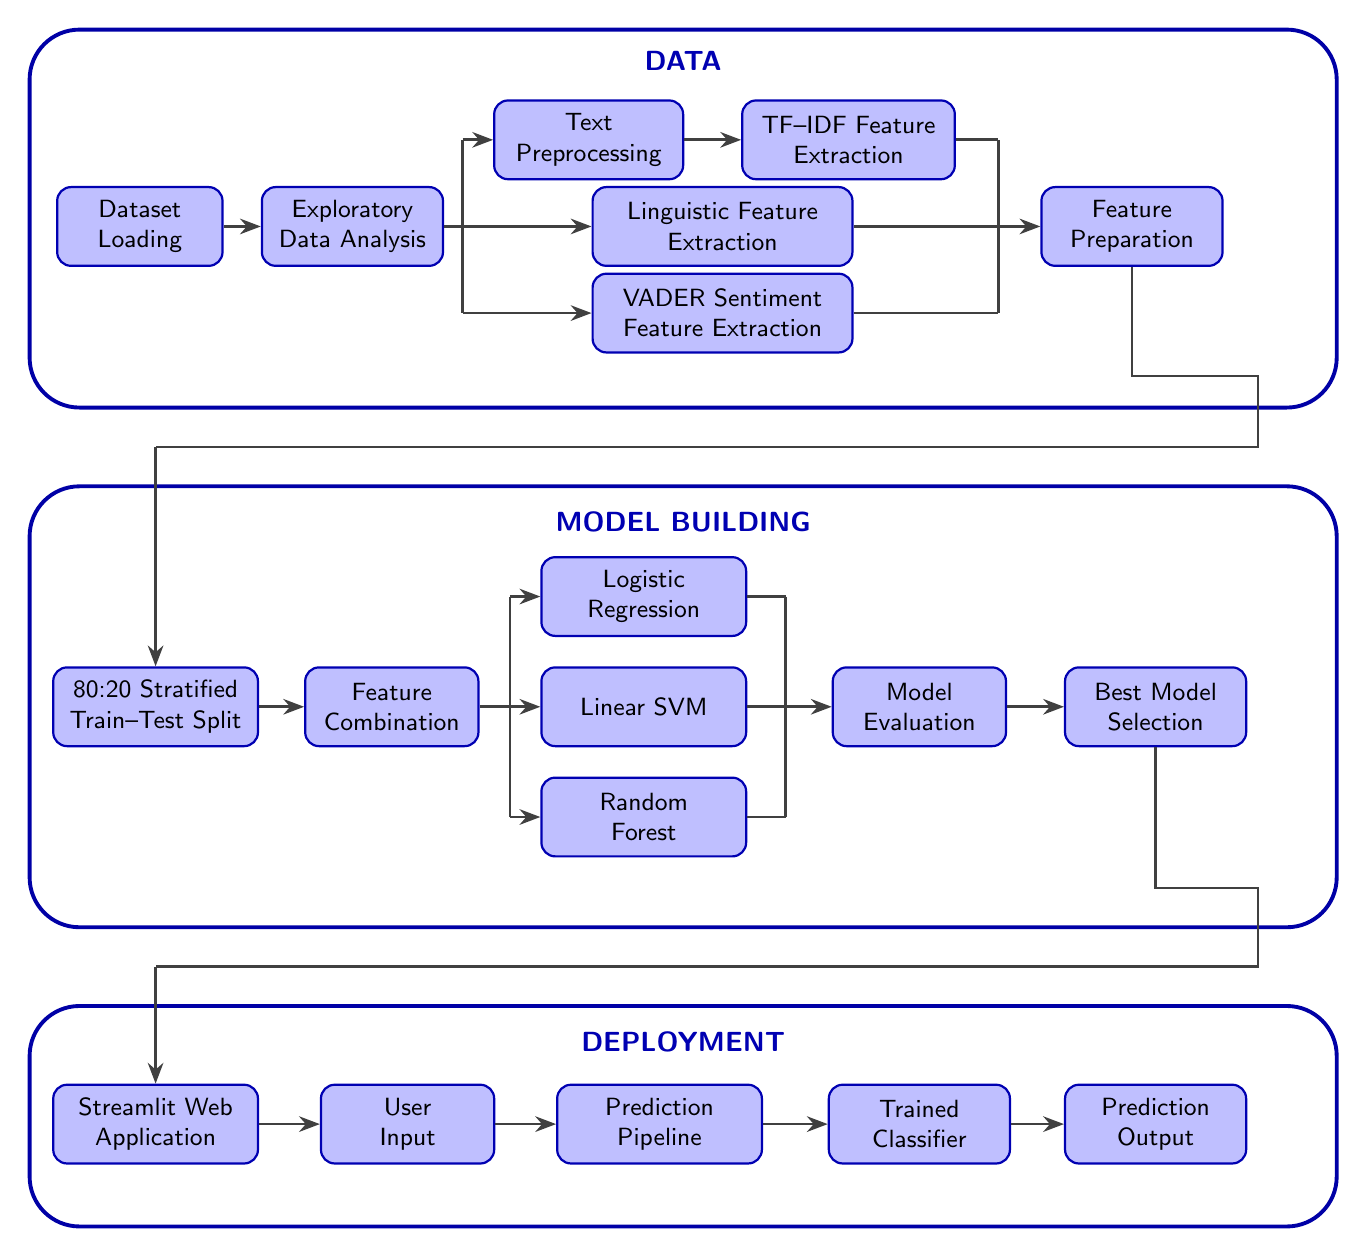
\begin{tikzpicture}[
    font=\sffamily\small,
    >=Stealth,
    % Outer Container Style (Width: 16.6cm)
    container/.style={
        draw=blue!65!black,
        line width=1.4pt,
        rounded corners=18pt,
        fill=white
    },
    container title/.style={
        font=\sffamily\bfseries\normalsize,
        text=blue!70!black
    },
    % Process Box Style
    block/.style={
        rectangle,
        draw=blue!70!black,
        fill=blue!25!white,
        line width=0.8pt,
        rounded corners=5pt,
        align=center,
        inner sep=4pt,
        minimum height=10mm,
        text=black
    },
    arrow/.style={
        ->,
        line width=1pt,
        draw=gray!50!black
    },
    link/.style={
        line width=1pt,
        draw=gray!50!black
    }
]

% =========================================================================
% CONTAINER 1: DATA
% Exact container bounds: (0.2, 0.0) to (16.8, 4.8)
% =========================================================================
\draw[container] (0.2, 0.0) rectangle (16.8, 4.8);
\node[container title] at (8.5, 4.4) {DATA};

% Nodes inside Container 1
\node[block, minimum width=2.1cm] (loading) at (1.6, 2.3) {Dataset\\Loading};
\node[block, minimum width=2.3cm] (eda) at (4.3, 2.3) {Exploratory\\Data Analysis};

\node[block, minimum width=2.4cm] (pre) at (7.3, 3.4) {Text\\Preprocessing};
\node[block, minimum width=2.7cm] (tfidf) at (10.6, 3.4) {TF--IDF Feature\\Extraction};

\node[block, minimum width=3.3cm] (ling) at (9.0, 2.3) {Linguistic Feature\\Extraction};
\node[block, minimum width=3.3cm] (vader) at (9.0, 1.2) {VADER Sentiment\\Feature Extraction};

\node[block, minimum width=2.3cm] (prep) at (14.2, 2.3) {Feature\\Preparation};

% Arrows inside Container 1
\draw[arrow] (loading) -- (eda);

% Fork bus from EDA (at x = 5.7)
\draw[link] (eda.east) -- (5.7, 2.3);
\draw[link] (5.7, 3.4) -- (5.7, 1.2);
\draw[arrow] (5.7, 3.4) -- (pre.west);
\draw[arrow] (pre) -- (tfidf);
\draw[arrow] (5.7, 2.3) -- (ling.west);
\draw[arrow] (5.7, 1.2) -- (vader.west);

% Join bus to Feature Preparation (at x = 12.5)
\draw[link] (tfidf.east) -- (12.5, 3.4);
\draw[link] (ling.east) -- (12.5, 2.3);
\draw[link] (vader.east) -- (12.5, 1.2);
\draw[link] (12.5, 3.4) -- (12.5, 1.2);
\draw[arrow] (12.5, 2.3) -- (prep.west);


% =========================================================================
% CONTAINER 2: MODEL BUILDING
% Exact container bounds: (0.2, -6.6) to (16.8, -1.0)
% =========================================================================
\draw[container] (0.2, -6.6) rectangle (16.8, -1.0);
\node[container title] at (8.5, -1.45) {MODEL BUILDING};

% Nodes inside Container 2
\node[block, minimum width=2.6cm] (split) at (1.8, -3.8) {80:20 Stratified\\Train--Test Split};
\node[block, minimum width=2.2cm] (comb) at (4.8, -3.8) {Feature\\Combination};

% 3 Parallel Candidate Models
\node[block, minimum width=2.6cm] (lr) at (8.0, -2.4) {Logistic\\Regression};
\node[block, minimum width=2.6cm] (svm) at (8.0, -3.8) {Linear SVM};
\node[block, minimum width=2.6cm] (rf) at (8.0, -5.2) {Random\\Forest};

\node[block, minimum width=2.2cm] (eval) at (11.5, -3.8) {Model\\Evaluation};
\node[block, minimum width=2.3cm] (best) at (14.5, -3.8) {Best Model\\Selection};

% Connectors inside Container 2
\draw[arrow] (split) -- (comb);

% Distribution bus (at x = 6.3)
\draw[link] (comb.east) -- (6.3, -3.8);
\draw[link] (6.3, -2.4) -- (6.3, -5.2);
\draw[arrow] (6.3, -2.4) -- (lr.west);
\draw[arrow] (6.3, -3.8) -- (svm.west);
\draw[arrow] (6.3, -5.2) -- (rf.west);

% Collection bus (at x = 9.8)
\draw[link] (lr.east) -- (9.8, -2.4);
\draw[link] (svm.east) -- (9.8, -3.8);
\draw[link] (rf.east) -- (9.8, -5.2);
\draw[link] (9.8, -2.4) -- (9.8, -5.2);
\draw[arrow] (9.8, -3.8) -- (eval.west);

\draw[arrow] (eval) -- (best);


% =========================================================================
% CONTAINER 3: DEPLOYMENT
% Exact container bounds: (0.2, -10.4) to (16.8, -7.6)
% =========================================================================
\draw[container] (0.2, -10.4) rectangle (16.8, -7.6);
\node[container title] at (8.5, -8.05) {DEPLOYMENT};

% 5 Balanced Nodes inside Container 3
\node[block, minimum width=2.6cm] (app) at (1.8, -9.1) {Streamlit Web\\Application};
\node[block, minimum width=2.2cm] (user) at (5.0, -9.1) {User\\Input};
\node[block, minimum width=2.6cm] (pipe) at (8.2, -9.1) {Prediction\\Pipeline};
\node[block, minimum width=2.3cm] (clf) at (11.5, -9.1) {Trained\\Classifier};
\node[block, minimum width=2.3cm] (pred) at (14.5, -9.1) {Prediction\\Output};

% Direct Sequential Arrows inside Container 3
\draw[arrow] (app) -- (user);
\draw[arrow] (user) -- (pipe);
\draw[arrow] (pipe) -- (clf);
\draw[arrow] (clf) -- (pred);


% =========================================================================
% INTER-CONTAINER CONNECTIONS (Drawn here because all nodes are now declared!)
% =========================================================================
% Route 1: From Feature Preparation to 80:20 Stratified Train-Test Split
\draw[link] (prep.south) -- (14.2, 0.4) -- (15.8, 0.4) -- (15.8, -0.5) -- (1.8, -0.5);
\draw[arrow] (1.8, -0.5) -- (split.north);

% Route 2: From Best Model Selection to Streamlit Web Application
\draw[link] (best.south) -- (14.5, -6.1) -- (15.8, -6.1) -- (15.8, -7.1) -- (1.8, -7.1);
\draw[arrow] (1.8, -7.1) -- (app.north);

\end{tikzpicture}
\end{document}
